\section{System Description}\label{sec:system}
The system architecture of \dReach{} is given in Figure~\ref{sec:system}. We ask the user to provide the following input file and two parameters:
\begin{itemize}
\item The input file specifies the hybrid system, the reachability
  properties in question, and some time bounds on the continuous flow in each mode.
  The grammar is described in
  Section~\ref{sec:input-format}.
\item A bound on the number of mode changes.
\item A numerical error bound $\delta$.%, as explained in Section A5. in the Appendix.
\end{itemize}
From these inputs, \dReach{} generates a logical encoding that involves existential quantification and universal quantification on the time variables. The logical encoding is compact, always linear in the size of the inputs. The tool then makes iterative calls to the underlying solver \dReal{}~\cite{DBLP:conf/cade/GaoKC13} to decide the reachability properties. When the answer is {\sf $\delta$-reachable}, \dReach{} generates a counterexample and its visualization. When the answer is {\sf unreachable}, no numerical error is involved and a (partial, for now) logical proof of unsatisfiability can be provided~\cite{SYNASC14}.
\begin{figure}[t]
  \centering
  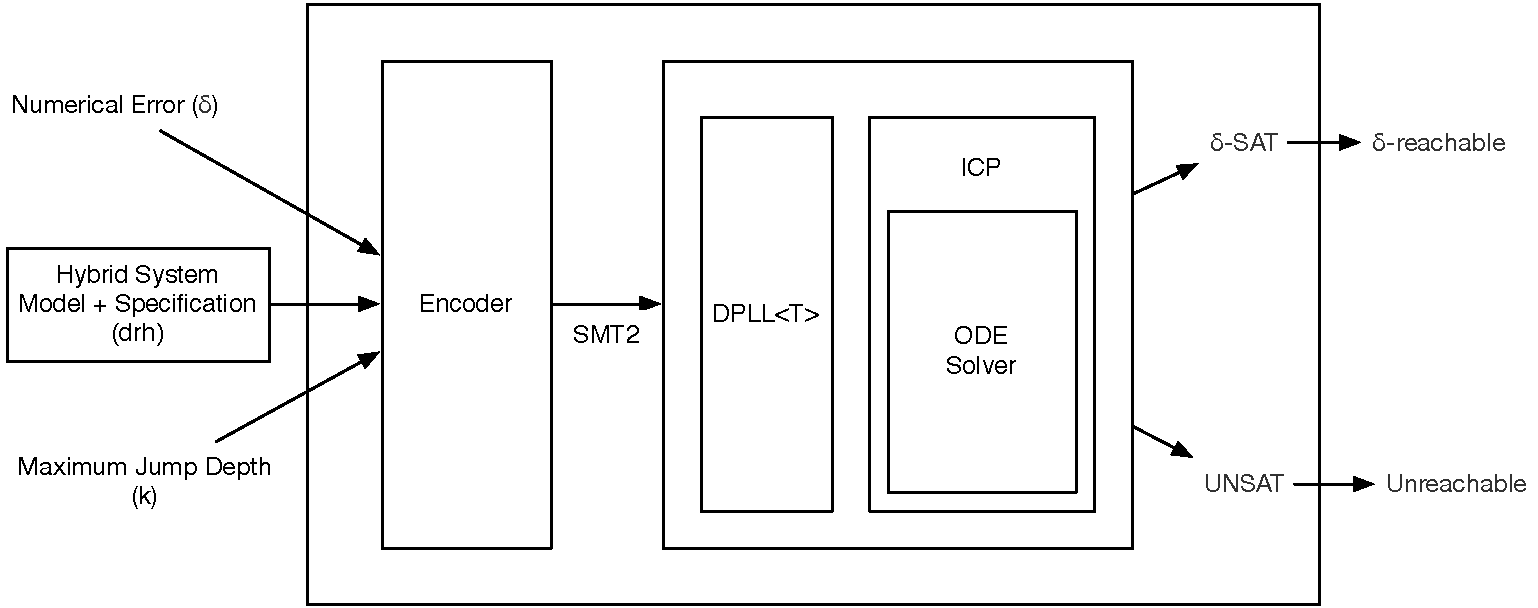
\includegraphics[width=\textwidth]{images/dreach_archi}
  \caption{Architecture of \dReach{}: It consists of an bounded
    model-checking module and an SMT solver, \dReal{}. In the first
    phase, the Encoder module translates an input hybrid system into a
    logic formula. In the second phase, an
    SMT solver, \dReal{}, solves the encoded $\delta$-reachability
    problem using a solving framework that combines DPLL(T), Interval Constraint Propagation, and reliable (interval-based) numerical integration.
  }\label{fig:system-description}
\end{figure}



%%% Local Variables:
%%% mode: latex
%%% TeX-master: "main"
%%% End:
